%%
% The BIThesis Template for Bachelor Graduation Thesis
%
% 北京理工大学毕业设计(论文)第二章节 —— 使用 XeLaTeX 编译
%
% Copyright 2020-2023 BITNP
%
% This work may be distributed and/or modified under the
% conditions of the LaTeX Project Public License, either version 1.3
% of this license or (at your option) any later version.
% The latest version of this license is in
%   http://www.latex-project.org/lppl.txt
% and version 1.3 or later is part of all distributions of LaTeX
% version 2005/12/01 or later.
%
% This work has the LPPL maintenance status `maintained'.
%
% The Current Maintainer of this work is Feng Kaiyu.
%%

\chapter{以出租车调度系统为背景的树状区块链测试}

\section{树状区块链上的出租车调度系统测试简介}

树状区块链将单链结构转化为树状结构的改进,提升了区块链技术在地理位置有关的应用场景下的理论效率。但实验室尚未对树状区块链在实际应用环境中的表现进行测试。因此,测试树状区块链在实际应用中的真实性能,证明其相较传统单链结构区块链具有可观性能提升的工作迫在眉睫。本章将以实验室已有工作——基于区块链的出租车调度系统为应用背景,以第二章的该系统的复现实验为基础,使用geth1和geth-tree分别构建不同拓扑结构的区块链并于其上运行该调度系统,统计在一定压力负载下司机侧和乘客侧各关键节点的时间戳并将结果可视化,以测试树状区块链在实际应用场景中的性能表现。同时,重构已有脚本的代码,增强其可扩展性和易用性,方面后人进行本测试的复现。

\section{测试设计思路}

本测试分为基于树状区块链geth-tree的测试和基于区域索引区块链geth1的测试两部分,用以对比两种区块链实现在同一套系统下的性能表现差异。

两部分实验中均在真实世界地图中Geohash编码前缀为wx4e的区域下进行。树状区块链部分的实验在该区域下的细分区域wx4en、wx4ep、wx4eq和wx4er区域下进行。每个区域中,均存在16位司机和32位乘客,所有司机的初始位置均相同,所有乘客的出发地点和目的地也相同。以上地点的选点工作基于蒙思洁完成的真实地图信息提取与筛选工作进行,已提前确保选择的路线可以在真实世界地图上导航成功。

本测试使用JavaScript脚本模拟司乘交互行为。司机模拟脚本负责读取司机的公钥地址、初始位置,并将其上传到链上;随后,司机将监听一系列合约中定义的事件,例如乘车请求事件、乘客上车事件和付款事件等,并作出接单、导航、设置车辆状态等响应。乘客模拟脚本负责读取乘客的公钥地址、起始点位置和目的地位置,并将其上传到链上;每隔一段时间(在树状区块链中为3秒,在区域索引区块链中为前者的$\frac14$),将有一名乘客发射乘车请求事件。发射乘车请求事件后乘客将在临近区域周边搜索与自身曼哈顿距离最近的车辆并尝试占有。若车辆已被占用,则等待一段时间(等待时间为冲突次数的一次函数)后再次重复上述步骤,直至车辆分配成功。乘客端、司机端的模拟脚本运行逻辑可分别用图\ref{乘客端模拟脚本运行逻辑}、图\ref{司机端模拟脚本运行逻辑}所示之流程图表示。

\begin{figure}[htbp]
    \centering
    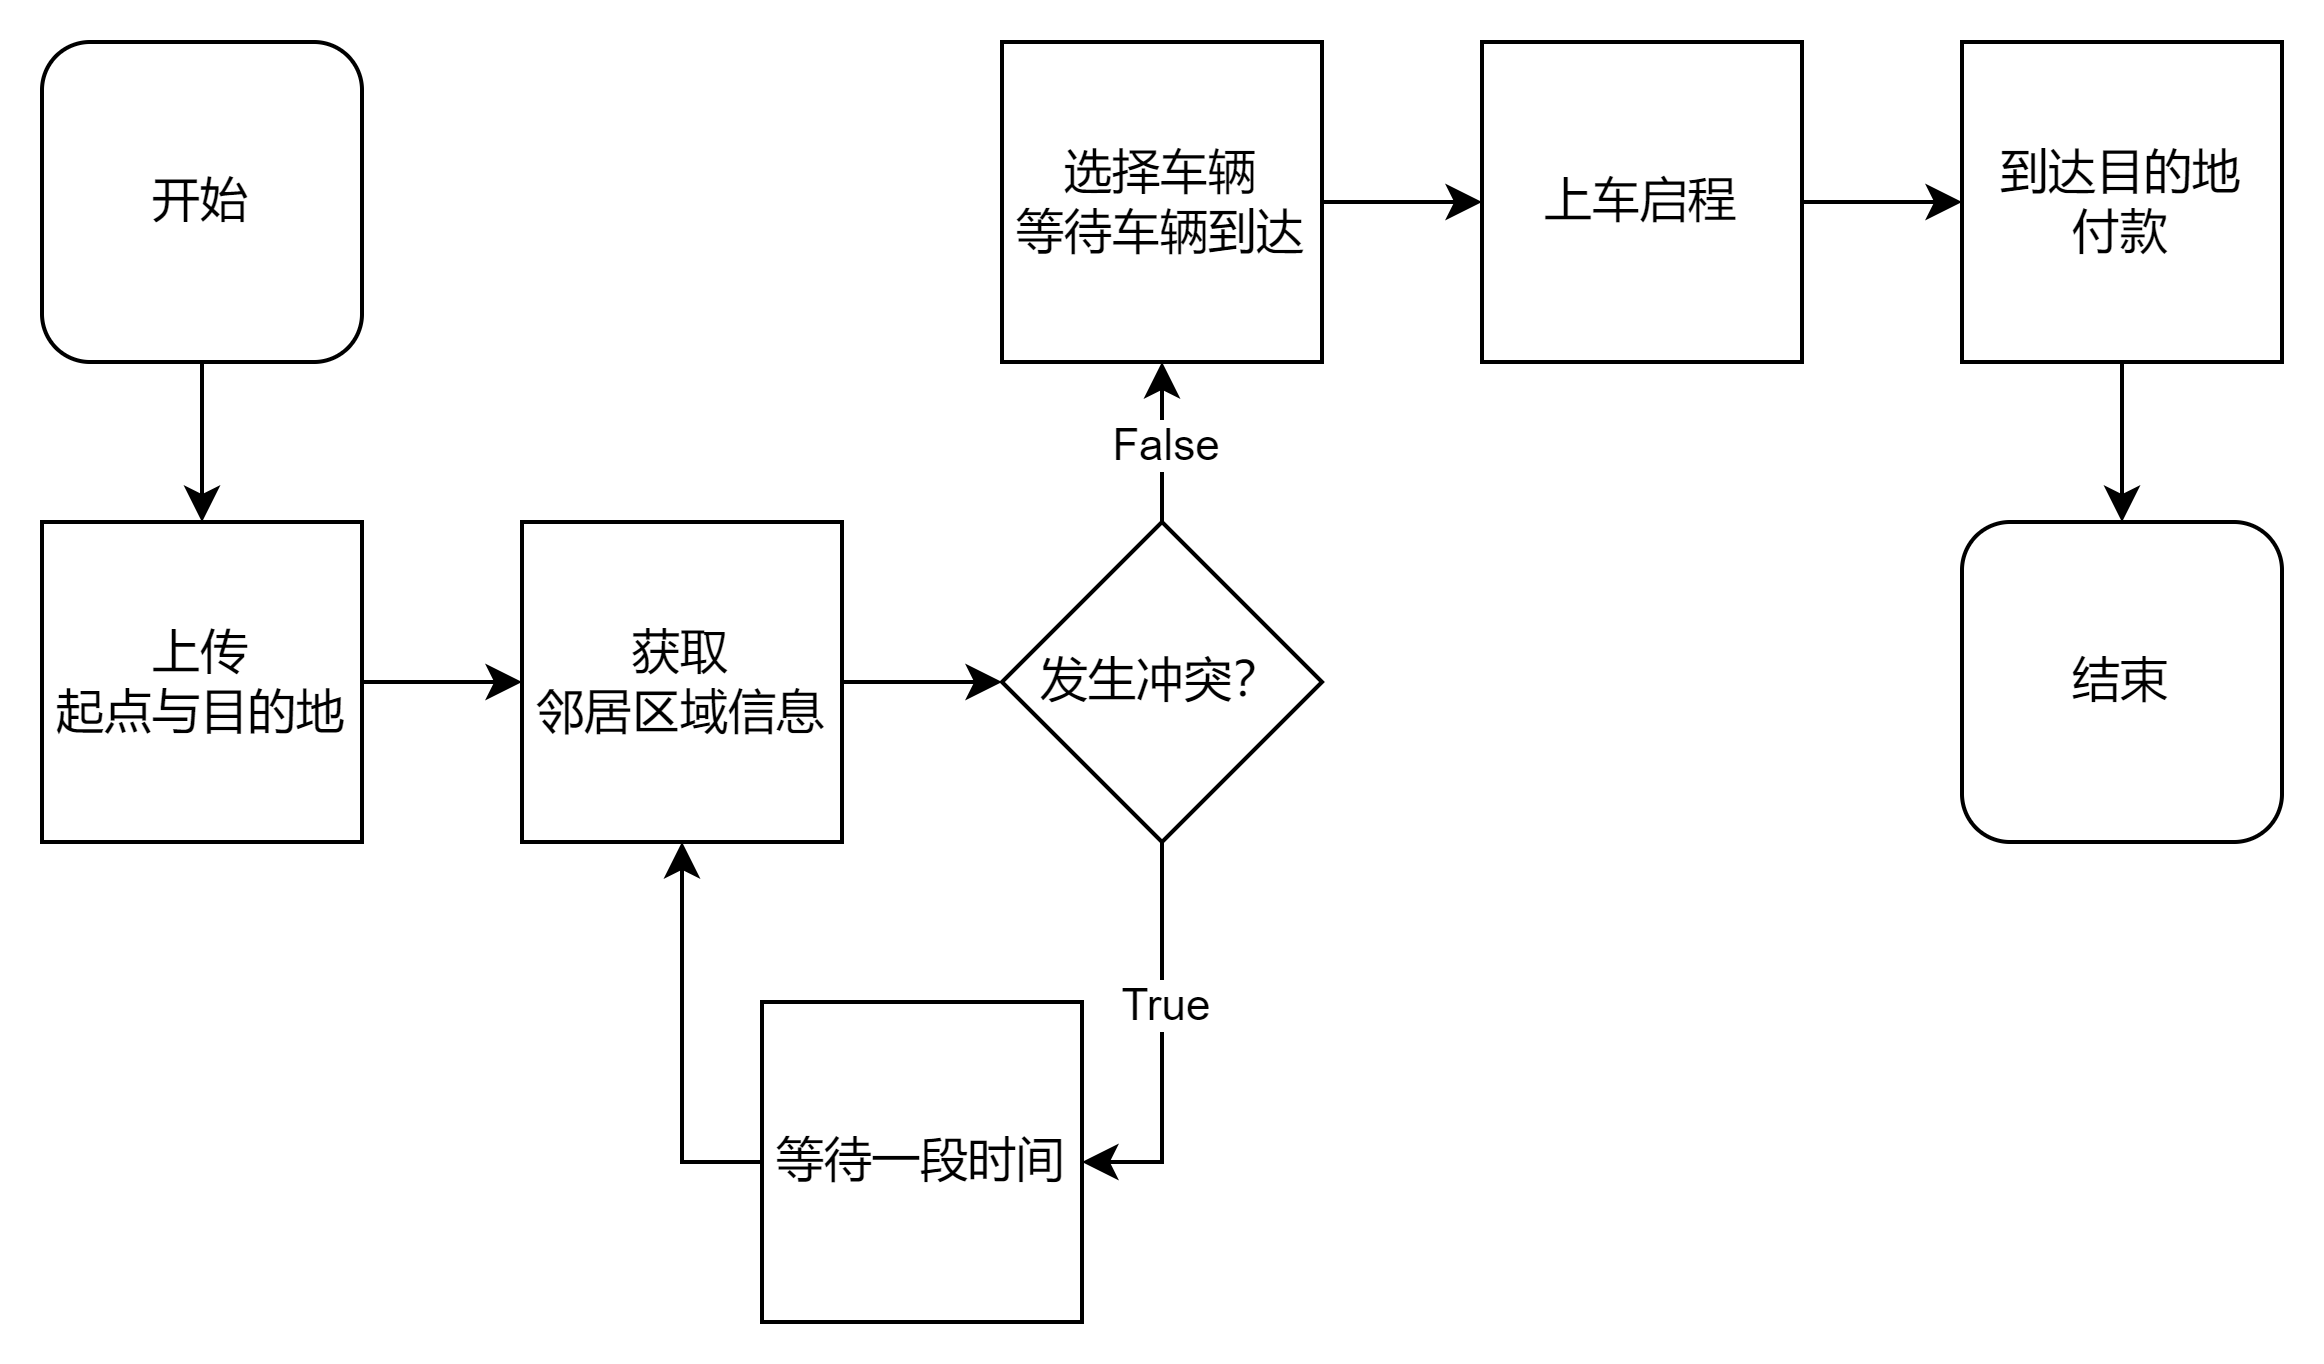
\includegraphics[width=\textwidth]{images/passenger示意图.png}
    \caption{乘客端模拟脚本运行逻辑}\label{乘客端模拟脚本运行逻辑} % label 用来在文中索引
\end{figure}

\begin{figure}[htbp]
    \centering
    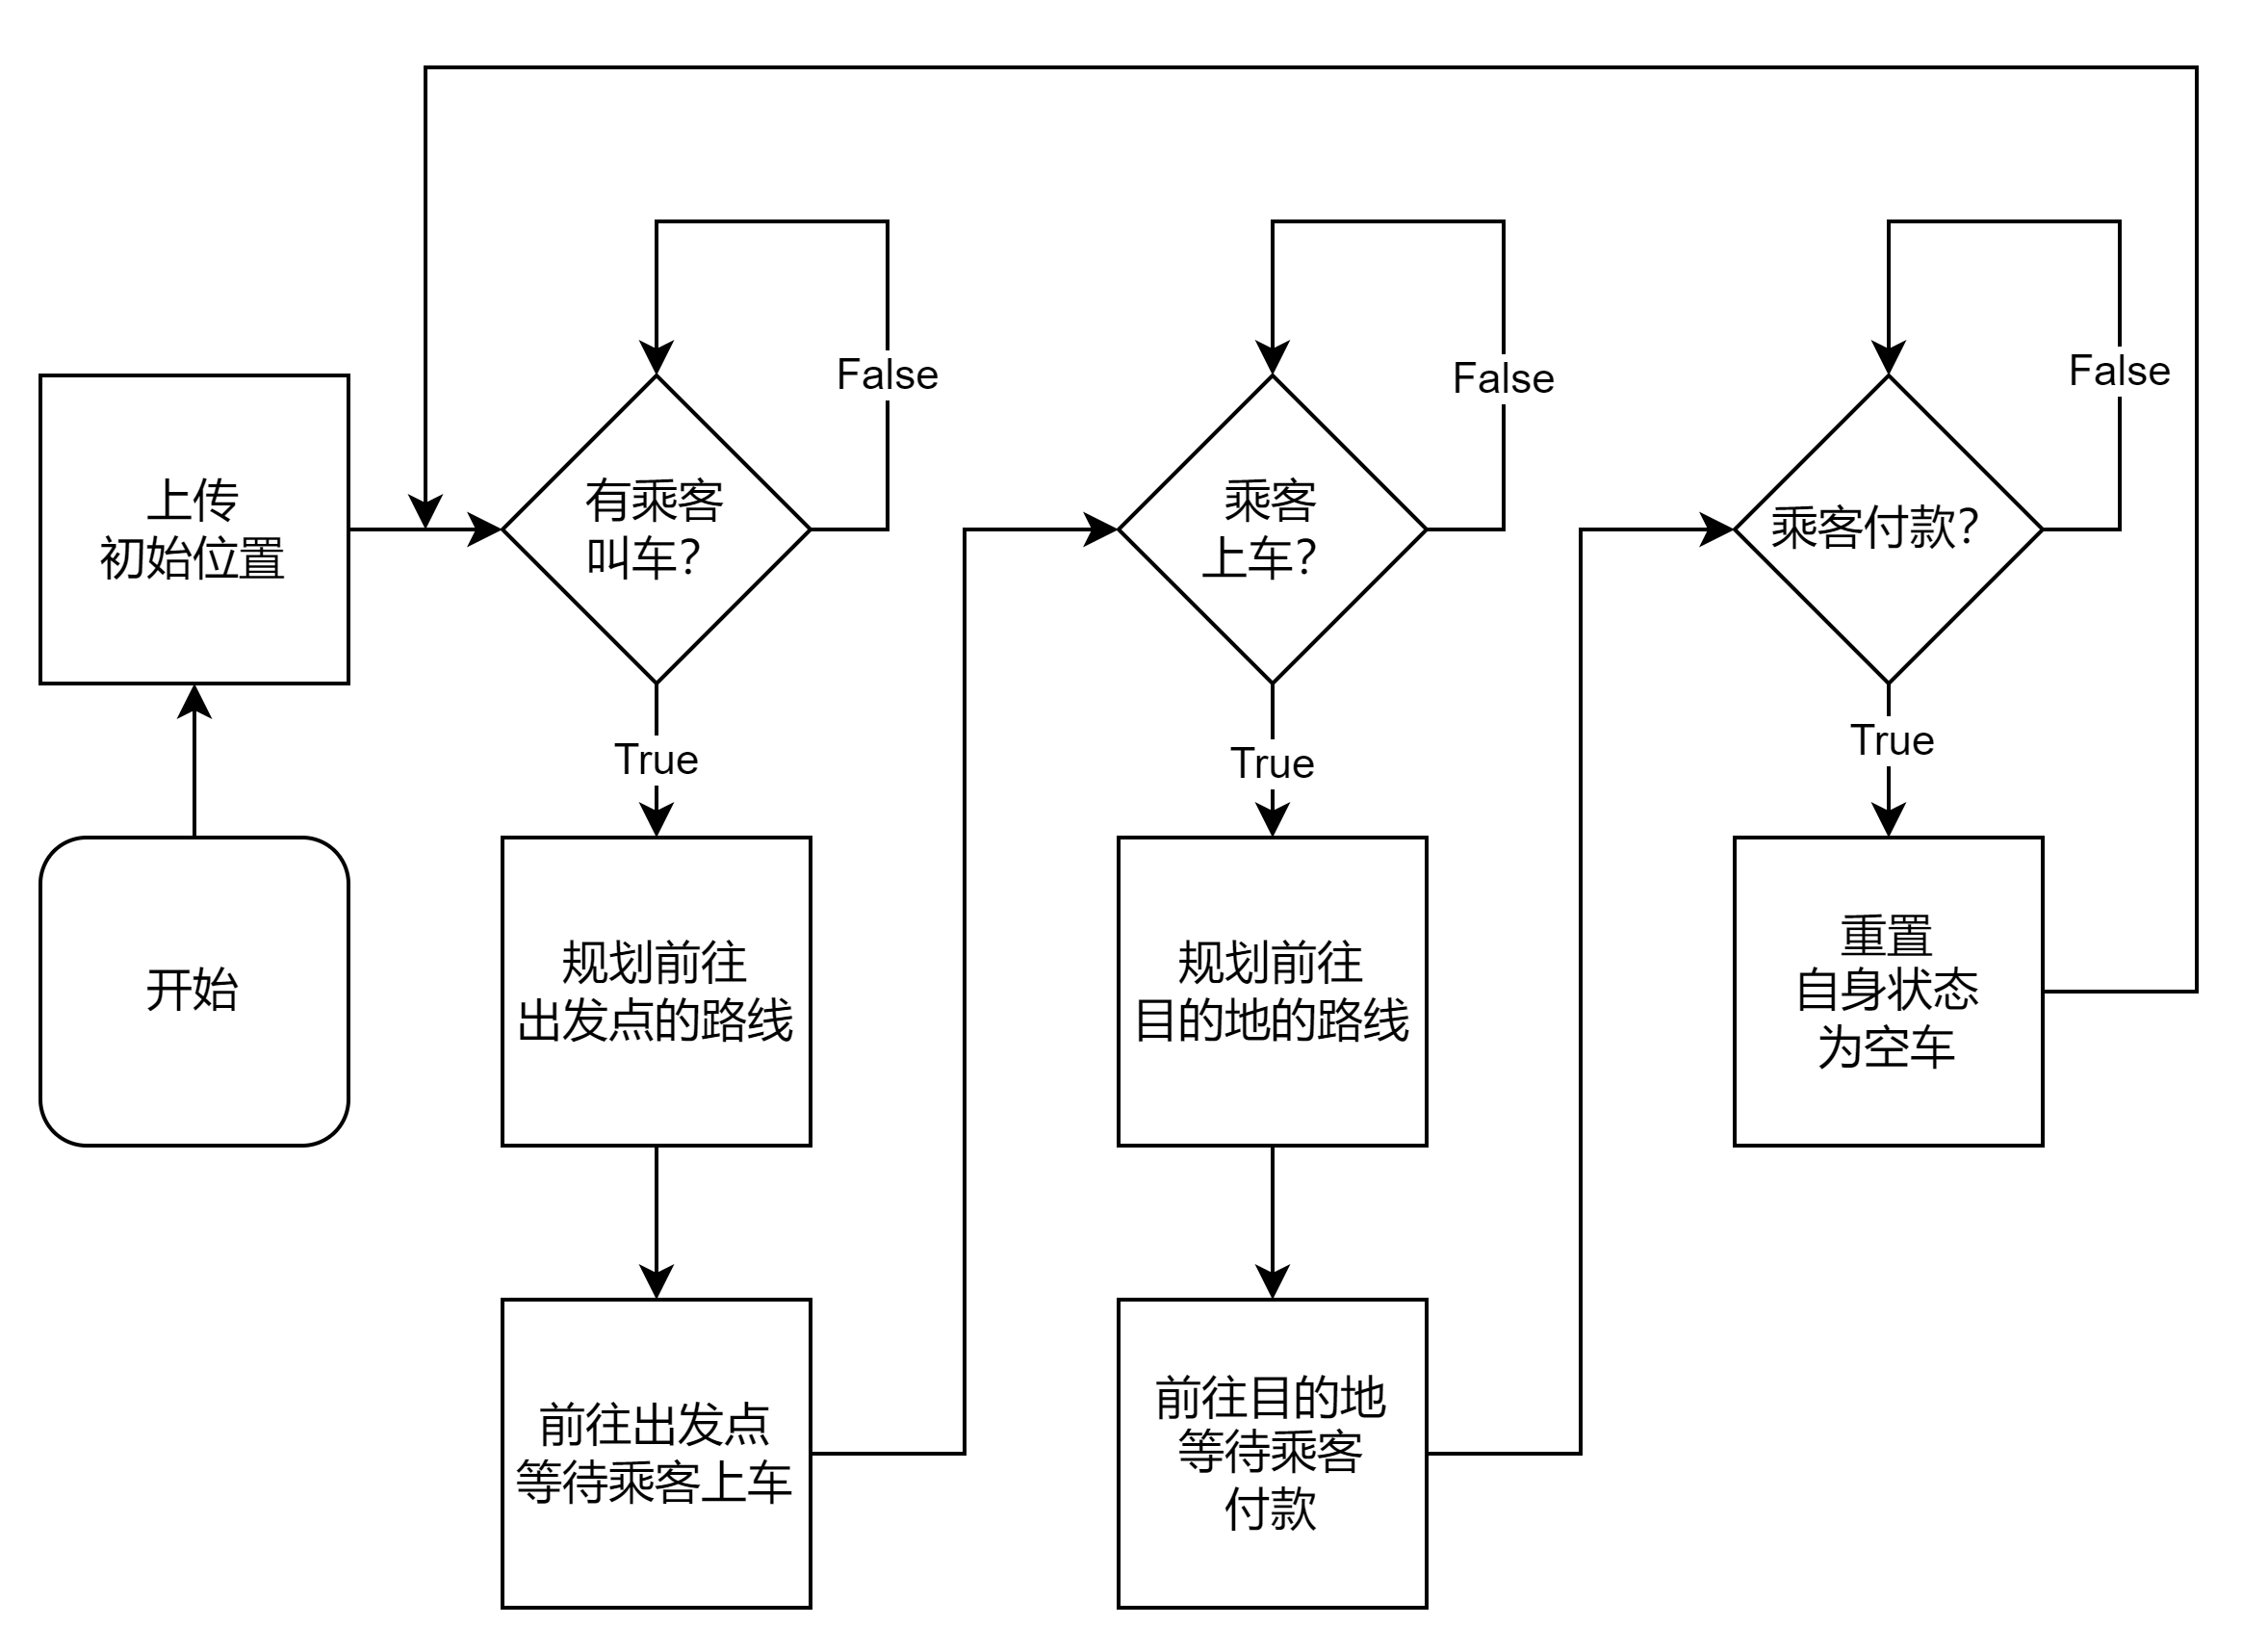
\includegraphics[width=\textwidth]{images/vehicle示意图.png}
    \caption{司机端模拟脚本运行逻辑}\label{司机端模拟脚本运行逻辑} % label 用来在文中索引
\end{figure}

进行树状区块链部分的实验时,首先搭建树状结构,在每个子链上分别部署合约。待合约部署完毕后,所有子链同时挖矿,并同时运行模拟司乘交互行为的JavaScript脚本,该脚本读取对应子链管辖的细分区域内的司乘信息,并记录司乘双方各自在调度过程关键节点的时间戳。

在区域索引区块链测试部分中,测试步骤大致相同,但运行司乘交互模拟脚本时,应令其读取所有四个细分区域内所司乘的信息,模拟不进行区域细分,使用单链结构区块链运行出租车调度系统的应用场景。

\section{测试环境}

基于树状区块链的调度系统测试在表\ref{树状区块链调度系统测试环境}环境中进行。由于运行四子链的性能开销较大,笔者使用Windows下的Linux子系统(WSL 2)代替虚拟机,以提升开发体验。

\begin{table}[htbp]
    \linespread{1.5}
    \zihao{5}
    \centering
    \caption{树状区块链调度系统测试环境}\label{树状区块链调度系统测试环境}
    \begin{tabular}{r|l} \toprule
        中央处理器 & Intel Core i5-12500H      \\
        图形处理器 & Intel Iris Xe 80EU        \\
        内存    & 24GB                      \\
        操作系统  & Ubuntu 22.04.2 LTS        \\
        虚拟机   & Windows Subsystem Linus 2 \\
        \bottomrule
    \end{tabular}
\end{table}

\section{准备数据}

\subsection{确定司乘位置信息}

本节将分别在各树状区块链子链的管辖区域内,为接下来的测试选择一条能够导航成功的路线,其始端和终端分别作为乘客的起点与目的地;司机的初始位置,则设置为乘客的目的地,即导航路线的终端。经过挑选和在调度系统中的验证工作后,笔者最终选择表\ref{测试数据集选点}中所示之点位,作为本章测试的测试数据集。

\begin{table}[htbp]
    \linespread{1.5}
    \zihao{5}
    \centering
    \caption{测试数据集选点}\label{测试数据集选点}
    \begin{tabular}{c|c|c|c} \toprule
        区域Geohash前缀 & 乘客起点        & 乘客终点        & 司机初始位置      \\\hline
        wx4en       & wx4enscgue5 & wx4enrq9mm9 & wx4enrq9mm9 \\
        wx4ep       & wx4epb8scg1 & wx4ep8e5gw0 & wx4ep8e5gw0 \\
        wx4eq       & wx4eq7rgmxk & wx4eqt6u0vu & wx4eqt6u0vu \\
        wx4er       & wx4erd4xkyz & wx4erw9rmze & wx4erw9rmze \\
        \bottomrule
    \end{tabular}
\end{table}

\subsection{划分账号扮演的角色}

基于区块链的出租车调度系统中,账号可以扮演司机或乘客角色。本测试共有192个账号参与其中,且司机角色与乘客角色的数量之比为$1:2$。不仅如此,测试还需保证在四条子链中包含相同数量的司机账号和乘客账号,以维护子链之间的测试公平性。经过计算,本测试将如表\ref{测试账号角色划分}所示,对链上创建的共计192个账号(表中以\verb|eth.accounts|指代)进行划分,该划分方案恰好满足所有子链包含相同数量的乘客账号和司机账号的测试需求。

\begin{table}[htbp]
    \linespread{1.5}
    \zihao{5}
    \centering
    \caption{测试账号角色划分}\label{测试账号角色划分}
    \begin{tabular}{l|l|l} \toprule
        区域Geohash前缀 & 司机账号                                & 乘客账号                                \\\hline
        wx4en       & \verb|eth.accounts.slice(0, 16)|    & \verb|eth.accounts.slice(16, 48)|   \\
        wx4ep       & \verb|eth.accounts.slice(48, 64)|   & \verb|eth.accounts.slice(64, 96)|   \\
        wx4eq       & \verb|eth.accounts.slice(96, 112)|  & \verb|eth.accounts.slice(112, 144)| \\
        wx4er       & \verb|eth.accounts.slice(144, 160)| & \verb|eth.accounts.slice(160, 192)| \\
        \bottomrule
    \end{tabular}
\end{table}

上述划分方案及各账号相关的位置信息将以JSON格式存储到文件,供模拟运行脚本读取之用。

\section{进行模拟运行测试}

本节的详细测试步骤已记录于在线代码仓库\footnote{\url{https://gitcode.net/qq_39710999/taxi-4-leaves}},故本节仅简要介绍大致测试方法。

\begin{enumerate}
    \item 准备司乘数据,使用JSON格式存储每位司乘的信息,并将其均匀分作4份,作为树状区块链子链的测试数据;同时,准备一套存储完整司乘信息的文件,作为区域索引区块链的测试数据;
    \item 建立有四个子链的树状区块链网络,确保四个子链中均拥有相同的192个账号,并已经为它们执行解锁操作;
    \item 在四子链上分别部署合约,并使用得到的合约地址更新各脚本中存储的合约地址,随后上传地图;
    \item 依次启动子链挖矿,注意分配CPU核心数量相同以控制变量,随后选择冲突等待时间和冲突次数的一次函数为$t_{waiting} = 10000 + 4000 \times count$,其中$count$为冲突次数,编辑模拟司机与乘客交互行为的脚本后启动之,等待测试结束;
    \item 模拟脚本运行结束后,将生成测试报告,可对其进行数据处理和可视化;
    \item 建立仅包含一个节点的区域索引区块链网络,于其上进行相似的测试。
\end{enumerate}

\section{乘客端测试数据分析}

本节采用Python 3编程语言的MatPlotLib库作为数据可视化工具,从乘客端方面对收集的测试数据进行分析。

本测试统计三个指标:乘车请求提交耗时、车辆分配耗时和到达并付款耗时。上述三个指标与图4-1中的对应关系如下:

\begin{itemize}
    \item 乘车请求提交耗时:从“开始”开始计时,直至第一次执行“发生冲突?”检查的耗时;
    \item 车辆分配耗时:从第一次执行“发生冲突?”检查开始,直至运行至“选择车辆 等待车辆到达”的耗时;
    \item 到达并付款耗时:从“选择车辆 等待车辆到达”开始计时,直至“结束”的耗时。
\end{itemize}

应用上述指标规则,对乘客端测试数据进行计算和可视化处理,其可视化结果如图\ref{乘客端耗时对比(子链并行运行)}所示所示。

\begin{figure}[htbp]
    \centering
    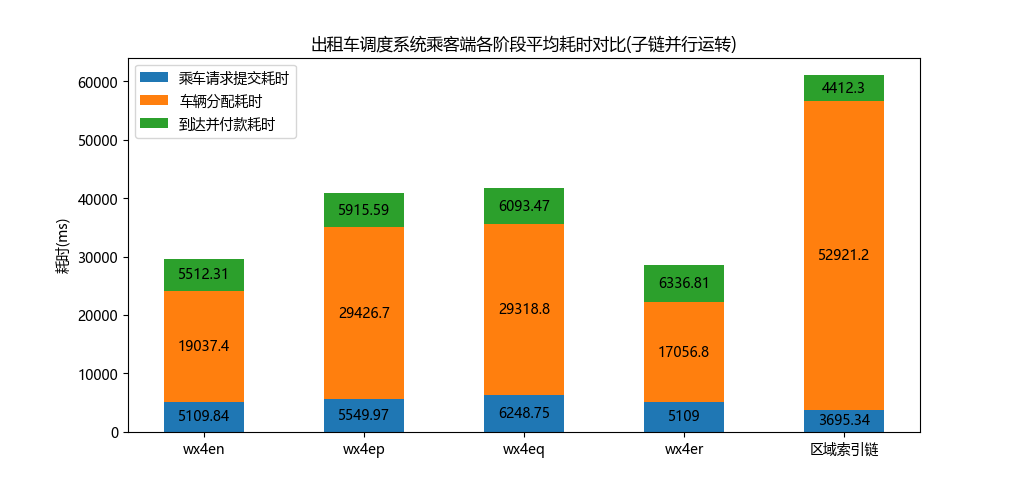
\includegraphics[width=\textwidth]{images/乘客端测试-并行.png}
    \caption{乘客端各阶段平均耗时对比(子链并行运转)}\label{乘客端耗时对比(子链并行运行)} % label 用来在文中索引
\end{figure}

分析图\ref{乘客端耗时对比(子链并行运行)}可知,树状区块链在为乘客分配车辆时,展现出了更为优越的性能。在该阶段中,树状区块链最快用时约17056.8毫秒即完成车辆分配,四子链平均车辆分配时间为23709.9毫秒;相比之下,区域索引区块链共耗时52921.2毫秒完成车辆分配,耗时增长至前者的2.23倍。

进一步分析测试报告发现,区域索引区块链上发生的冲突次数远远大于树状区块链中的各条子链上的冲突次数,是拖慢调度系统在其上运行速度的主要原因。测试报告指出,在区域索引区块链上,一共发生了266次这样的冲突事件;作为对比,冲突事件在wx4en子链、wx4ep子链、wx4eq子链和wx4er子链中的发生次数分别仅有18、31、33、12次,远低于区域索引区块链上的冲突次数。

\subsection{减少无关变量后的补充测试}

注意到,乘客方提交乘车请求、到达目的地并支付路费时,其处理速度相较区域索引区块链并未展现出更高的效率,耗时甚至不降反升。由于测试时四条子链并行运行,且笔者观察到测试时计算机中央处理器负载极高,一度达到满载,故做出如下合理推测:四条子链并行的测试方法极有可能受到测试机器性能上限之影响,从而引入无关变量,令测试数据失真。

为缓解测试机器性能上限对测试结果的影响,笔者补充进行了四次树状区块链实验,每次实验中,仅有一条子链单独运行模拟运行测试,其余三条子链空闲无负载。使用新方法重新测试后,子链的性能表现有了极大的提升,如图\ref{乘客端耗时对比(子链独立运行)}所示。

\begin{figure}[htbp]
    \centering
    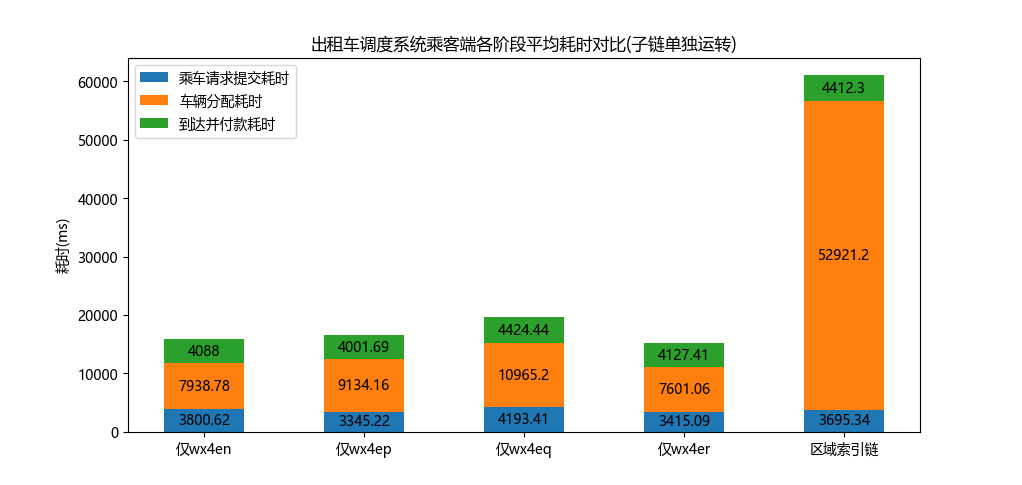
\includegraphics[width=\textwidth]{images/乘客端测试-独立.png}
    \caption{乘客端各阶段平均耗时对比(子链单独运转)}\label{乘客端耗时对比(子链独立运行)} % label 用来在文中索引
\end{figure}

在各个子链独立运行的场景下,测试机器的性能上限带来的影响进一步减弱,此时树状区块链爆发出了远超区域索引区块链的性能表现。在乘车请求提交平均耗时方面,树状区块链与区域索引区块链在该阶段的平均耗时基本一致;在车辆分配耗时方面,四条子链的平均耗时为8909.8毫秒,相较四子链并行运行的工况减少了62.4\%,相比区域索引区块链,其时间开销更是缩短到原来的16.8\%。在到达并付款耗时方面,由于调度系统运行至该阶段时,链上存在的区块数量已较有规模,树状区块链将区块分散至子链以换取更高的处理速度的优势得以提现,此时,四条子链的平均时间消耗为4160.4毫秒,以251.9毫秒的优势领先区域索引区块链。

\section{司机端测试数据分析}

本节使用与上一节相同的工具,对司机端方面进行测试数据分析。

本测试统计三个指标:接单并导航至上车点耗时、导航至目的地耗时和确认乘客下车并付款耗时耗时。上述三个指标与图\ref{乘客端模拟脚本运行逻辑}中的对应关系如下:

\begin{itemize}
    \item 接单并导航至上车点耗时:从“有乘客叫车”检查为真开始,至“前往出发点等待乘客上车”的耗时;
    \item 导航至目的地耗时:从“乘客上车”检查为真开始,至“前往目的地等待乘客付款”的耗时;
    \item 确认乘客下车并付款耗时:从“乘客付款”检查为真开始,至“重置自身状态为空车”为止。
\end{itemize}

应用上述指标规则,对司机端测试数据进行统计和可视化处理。此处沿用了乘客端测试的方法,同时测试了在四条子链并行运转和分别运转的工况下调度系统的运行情况。经过处理和汇总的数据可视化结果如图\ref{司机端平均耗时对比}所示所示。

\begin{figure}[htbp]
    \centering
    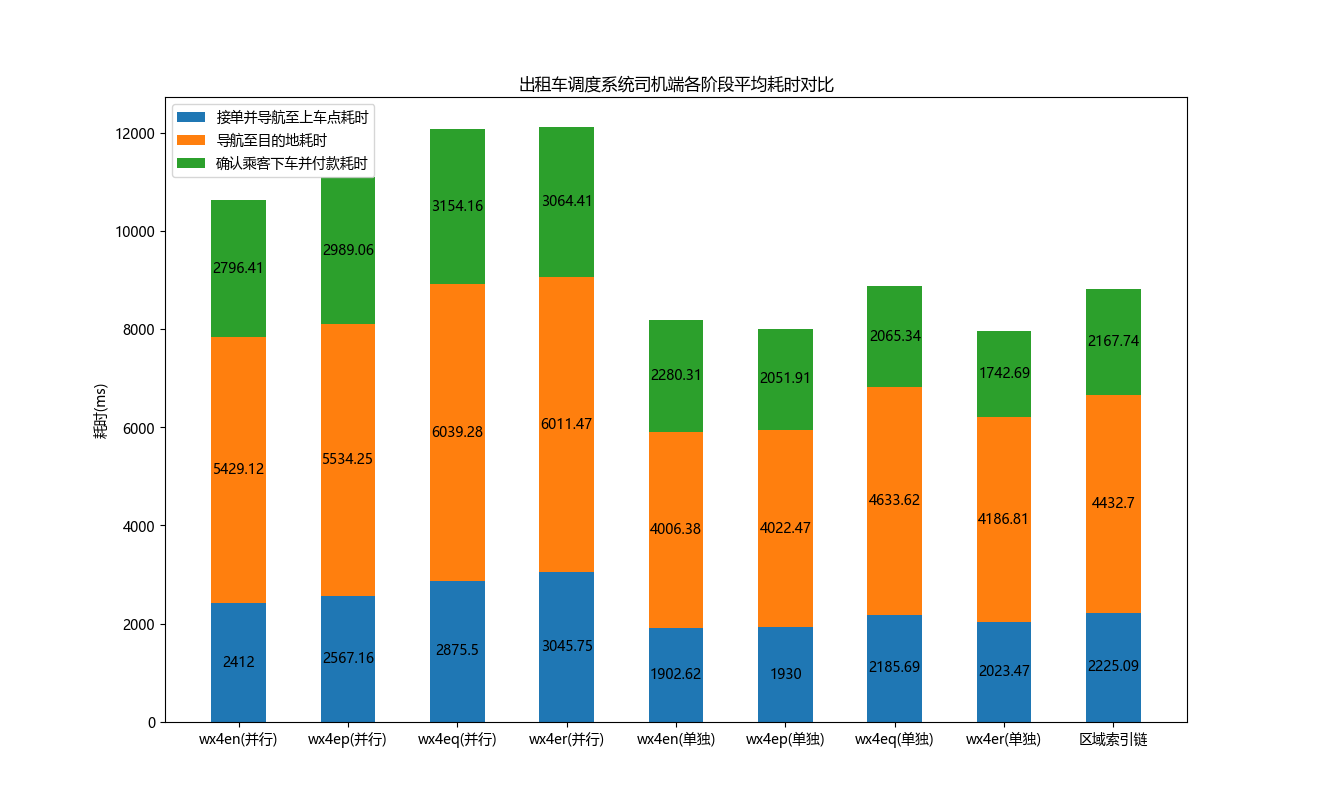
\includegraphics[width=\textwidth]{images/司机端测试.png}
    \caption{出租车调度系统司机端各阶段平均耗时对比}\label{司机端平均耗时对比} % label 用来在文中索引
\end{figure}

由图\ref{司机端模拟脚本运行逻辑}可知,司机端不存在冲突的情况(即:系统不允许同一时间有两位司机接受同一位乘客的订单),加之并行运行为测试计算机带来的较大负担,在四子链并行运行的工况下,树状区块链的性能表现大幅落后于区域索引区块链。然而,在四子链分别单独运行,测试计算机性能影响因素被减弱的工况下,树状区块链仍然以567.7毫秒的平均周转耗时优势超越了单链结构的区域索引区块链。测试证明,树状区块链相较传统区块链的性能优势并非仅来自调度系统运行时产生的诸如冲突等特殊情况,其树状结构的物理设计功不可没。然而,四条子链同时运行产生的性能开销,有可能制约树状区块链的综合性能,令区块链网络的运行效率产生不可忽视的下降。

\section{本章小结}

本章介绍了树状区块链在基于区块链的出租车调度系统上进行的各项测试及其数据分析。首先,阐述了设计测试的思路及大致方法。本章测试在采用经过分块处理的真实世界地图的基础上,采用脚本模拟司机与乘客的交互行为,在具有四个叶子链的树状区块链系统上部署出租车调度系统合约并运行模拟脚本,以收集实验数据。接下来,展示了实验环境配置,及较具体的数据准备、模拟测试的步骤方法。最后两节分别从乘客端角度和司机端角度出发,选取了不同的性能指标进行统计分析,并将结果进行可视化。针对树状区块链优于传统区块链的情况,给出了直观的展示;针对树状区块链不及传统区块链的情况,则给出了测试平台性能上限的猜想,同时设计进行补充实验加以验证该猜想,最终获得了树状区块链在实际应用场景的不同工况下的性能表现,证明了它相较传统的单链结构区块链的性能优越性。同时,证明了测试平台性能上限对树状区块链运行的影响,解释了树状区块链提供更好性能的代价之一——对系统资源的占用情况较为严重。
